\chapter{Results}
\label{cha:results}
The next two sections will discuss the results of the two abstract components of this work: the \textit{Symptom Identifier} and the \textit{Symptom Classifier}.

\section{Evaluation of the Symptom Identifier}
\label{sec:eval_symptom_identifier}
In order to evaluate the Symptom Identifier, the tokens for predictions of each sentence were classified in four classes:
\begin{itemize}
  \item \texttt{correct} tokens: they contain an intelligible symptom that is also present in the patient's sentence;
  \item \texttt{redundant} tokens: when the token is correct but there is another token that has the same meaning;
  \item \texttt{non sense} tokens: they are not intelligible;
  \item \texttt{wrong} tokens: they are deceptive because they contain an intelligible symptom but that is not present in the patient's sentence.
\end{itemize}

For each sentence, the number of symptoms present in the sentence but not in the tokens were counted: \texttt{missing tokens}.

In order to choose the best model for future evaluations, a score metric that summarizes the performance of this component has been designed.\footnote{``\texttt{\#C}'' means ``total number of predictions belonging to the class \texttt{C}''}:
\begin{equation}
score = \texttt{\#correct} + 0 \cdot \texttt{\#redundant} - \texttt{\#non sense} - \texttt{\#wrong} - \texttt{\#missing}
\end{equation}

The \texttt{non sense} tokens have the same penalizing factor as the \texttt{wrong} ones because they may lead to a random prediction. Instead, a redundant token is neutral because it might lead to a duplicated, but correct, prediction.

Table \ref{tab:bertrnet} compares BERT and R-NET.

\definecolor{green}{rgb}{0.8,0.9,0.8}
\definecolor{lightgreen}{rgb}{0.89, 0.94, 0.89}
\definecolor{red}{rgb}{1,0.89,0.89}

\begin{center}
  \begin{table}
     \begin{tabular}{| c | c | c | c |} 
     \hline
     \# of & BERT & R-NET \\ [0.5ex] 
     \hline\hline
     \rowcolor{green}
     \texttt{correct} & 423 & 427 \\ 
     \hline
     \rowcolor{lightgreen}
     \texttt{redundant} & 275 & 195 \\
     \hline
     \rowcolor{red}
     \texttt{non sense} & 122 & 247 \\
     \hline
     \rowcolor{red}
     \texttt{wrong} & 8 & 14 \\
     \hline
     \rowcolor{red}
     \texttt{missing} & 61 & 74 \\
     \hline
     \textbf{score} & \textbf{232} & \textbf{92} \\ 
     \hline
    \end{tabular}
 \caption{\label{tab:bertrnet} Score comparison between BERT for QA and R-NET.}
 \end{table}
\end{center}

The results, and, in particular, the score measure, suggest that BERT is consistently better for this task. For this reason the outcome of BERT for QA was used as input for the evaluation of the Symptom Classifier.

In order to better visualize the outcome of BERT and R-NET, some more indices, shown in table \ref{moreindicesbertrnet}, has been calculated. These are:
\begin{enumerate}
  \item the fraction of \texttt{redundant} and \texttt{non-redundant correct tokens} over the total number of tokens;
  \item the fraction of \texttt{non-redundant correct tokens} over the total number of tokens;
  \item the fraction of \texttt{non-redundant correct tokens} over the sum of \texttt{non-redundant correct tokens} and \texttt{missing tokens}: it represents the percentage of identified symptoms.
\end{enumerate}

\newcolumntype{C}{ >{\centering\arraybackslash} m{4cm} }
\newcolumntype{D}{ >{\centering\arraybackslash} m{2cm} }
\begin{center}
 \begin{table}
     \begin{tabular}{| C | D | D |}
     \hline
     measures & BERT & R-NET \\ [1ex] 
     \hline\hline
     \texttt{$\frac{\texttt{\#correct} + \texttt{\#redundant}}{\texttt{\#TFP}}$} & 84.8 \% & 70.4 \% \\[1ex]
     \hline
     \texttt{$\frac{\texttt{\#correct}}{\texttt{\#TFP}}$} & 52.6 \% & 48.4 \% \\[1ex]
     \hline
     \texttt{$\frac{\texttt{\#correct}}{\texttt{\#correct} + \texttt{\#missings}}$} & 88.0 \% & 87.5 \% \\[1ex]
     \hline
    \end{tabular}
  \caption{\label{tab:moreindicesbertrnet} }
  \end{table}
\end{center}

The first index of table \ref{tab:moreindicesbertrnet} shows that BERT outperform R-NET by 14.4\%; however, the percentage of non-redundant correct tokens and the percentage of identified tokens are similar. This means that BERT produces more redundant correct tokens than R-NET, while R-NET outputs more non-sense tokens.

\section{Evaluation of the Symptom Classifier}
\label{sec:evalsymptomclassifier}
\subsection{Definitions and notation}
Some notation that will be used in the following sections:
\begin{itemize}
  \item $\texttt{real cuis}_{i}$: list of actual symptom CUIs of the i-th sentence;
  \item $\texttt{predicted cuis}_{i}$: list of predicted CUIs of the i-th sentence;
  \item \texttt{\#}: stands for ``number of''.
\end{itemize}

\subsubsection{Types of predictions}
The predictions can be classified as:
\begin{itemize}
  \item \texttt{correct}, if it is located in a subtree rooted in any of the \texttt{real cuis}. These can be of two types:
    \begin{itemize}
      \item \textit{redundant} (\texttt{R}). When a prediction is mapped to a subtree, the subtree is marked as associated with that prediction. Then, if another prediction of the same sentence stays in that subtree, it is classified as redundant;
      \item \textit{non-redundant} (\texttt{NR}), if the prediction stays in a unmarked subtree;
    \end{itemize}
  \item \texttt{wrong}, if the prediction is not located in any of the subtrees.
\end{itemize}

These terms are also contextual to the sentence: this means that they can be indexed as well. For instance, $\texttt{\#correct}_{i}$ represents the number of correct predictions of the i-th sentence.

\subsection{Measures}
The \textit{Symptom Classifier} performs a slight variation of multi-class classification: a class for each symptom present in the tree. The variation stands in the \textit{pruning} option because the number of candidate classes decreases, and in the fact that, if the predicted CUI and the real one are different (i.e. they are of different classes), the prediction could be correct (if it stays in the subtree of the real CUI).

Some new indices has been developed in order to evaluate the performance of this component:
\begin{enumerate}

  \item \texttt{accuracy}: it represents the fraction of symptoms that were predicted correctly over the total number of symptoms.
  \begin{equation}
  \texttt{accuracy} = \frac{\sum_{i}{\texttt{\#correct}_{i}^{\texttt{NR}}}}{\sum_{i}{\texttt{\#real cuis}_{i}}}
  \end{equation}

  \item \texttt{\% of correct predictions}: it is the fraction of the number of correct predictions (redundant and non-redundant) over the total number of predictions. It represents the probability, for a prediction, of being correct.
  \begin{equation}
  \texttt{\% of correct predictions} = \frac{\sum_{i}{\texttt{\#correct}_{i}}}{\sum_{i}{\texttt{\#predicted cuis}_{i}}}
  \end{equation}

  \item \texttt{medium attempts}: it is computed as the total number of predictions over the total number of actual symptoms present in the sentences and represents the medium number of attempts that the model does for each symptom a the sentence.
  \begin{equation}
  \texttt{medium attempts} = \frac{\sum_{i}{\texttt{\#predicted cuis}_{i}}}{\sum_{i}{\texttt{\#real cuis}_{i}}}
  \end{equation}

  \item \texttt{missed symptoms}: complementary to the \texttt{accuracy}, it can be useful to understand the number of missed tokens.
  \begin{equation}
  \texttt{missed symptoms} = \sum_{i}{\texttt{\#real cuis}_{i}} - \sum_{i}{\texttt{\#correct}^{\texttt{NR}}_{i}}
  \end{equation}

\end{enumerate}

%%%%%%%%%%\newpage
\subsection{Evaluation of different options}
\label{sec:evaluationoptions}
This subsection analyzes individually every option of the Symptom Classifier. These are: 
\begin{itemize}
  \item the embedding type
  \item \textit{Body Part Finder}
  \item ``pruning''
  \item the filter for ``useless words''
  \item \textit{minimum similarity} threshold

\subsubsection{Comparison of different types of embeddings}

\begin{figure}[h]%[!tbp]
  \centering
  \begin{minipage}[b]{0.4\textwidth}
    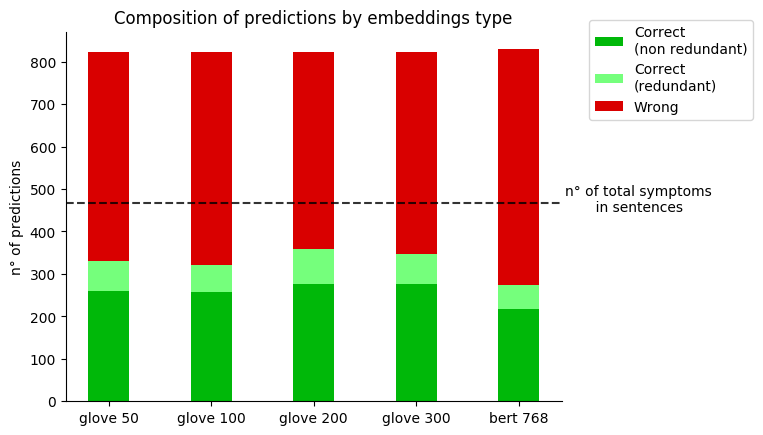
\includegraphics[width=9cm]{graphs/comparison_embeddings_type}
    \caption{Comparison of the composition of the predictions across different embedding types.}
  \end{minipage}
  \hfill
  \begin{minipage}[b]{0.4\textwidth}
    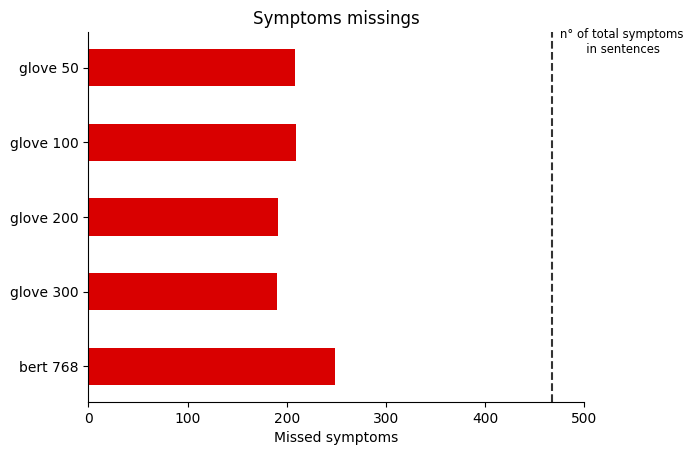
\includegraphics[width=8cm]{graphs/comparison_embeddings_type_missings}
    \caption{Comparison of the \texttt{missing symptoms} across different embedding types.}
  \end{minipage}
\end{figure}

\begin{center}
 \begin{tabular}{| c | c | c | c | c | c |} 
 \hline
 \thead{\texttt{embedding}\\\texttt{type}} & \thead{\texttt{accuracy}} & \thead{\texttt{correct}\\\texttt{predictions}} & \thead{\texttt{harmonic}\\\texttt{mean}} & \thead{\texttt{medium}\\\texttt{attempts}} & \thead{\texttt{missed}\\\texttt{symptoms}} \\ [0.5ex] 
 \hline\hline
 \texttt{GloVe 50} & 55.5 \% & 40.1 \% & 46.5 \% & 1.8 & 208 \\ 
 \hline
 \texttt{GloVe 100} & 55.2 \% & 39.1 \% & 45.8 \% & 1.8 & 209 \\
 \hline
 \texttt{GloVe 200} & 59.1 \% & 43.7 \% & 50.2 \% & 1.8 & 191 \\
 \hline
 \texttt{GloVe 300} & 59.3 \% & 42.2 \% & 49.3 \% & 1.8 & 190 \\
 \hline
 \texttt{BERT emb.} & 46.7 \% & 32.9 \% & 38.6 \% & 1.8 & 249 \\
 \hline
\end{tabular}
\caption{Comparison of different types of embeddings using different indices.}
\label{tab:comparison_emb}
\end{center}

%%%%%%%%%%%%%%%%%%%%%%%%%%% discuss data

During this test different types of embeddings were compared. As shown in table \ref{tab:comparison_emb}, the performances of \texttt{GloVe 50} and \texttt{GloVe 100} are very similar (considering, for example, the harmonic mean between accuracy and correct predictions). However, \texttt{GloVe 200} introduced an improvement compared to \texttt{GloVe 100} (+ 3.9 \% of accuracy and + 4.6 \% of correct predictions ). This trend is also confirmed by \texttt{GloVe 300} (+ 4.1 \% of accuracy and + 3.1 \% of correct predictions). Looking at these results, \texttt{GloVe 200} was chosen as the default embedding type used for the following tests.

The \texttt{medium attempts} are all equal because the options that cause a decrease of the number of predictions are not enabled: the Body Part Finder cause an increase of them and using zero level of minimum similarity does not affect the number of predictions.

BERT embeddings do not perform as good as GloVe embeddings: this is due to the fact that they were extracted from a non-finetuned BERT, which has not been trained on any medical corpus.

%%%%%%%%%%%%%%%%%%%%%%%%%%%
\newpage
\subsubsection{Ablation test for the Body Part Finder}

\begin{figure}[h]%[!tbp]
  \centering
  \begin{minipage}[b]{0.4\textwidth}
    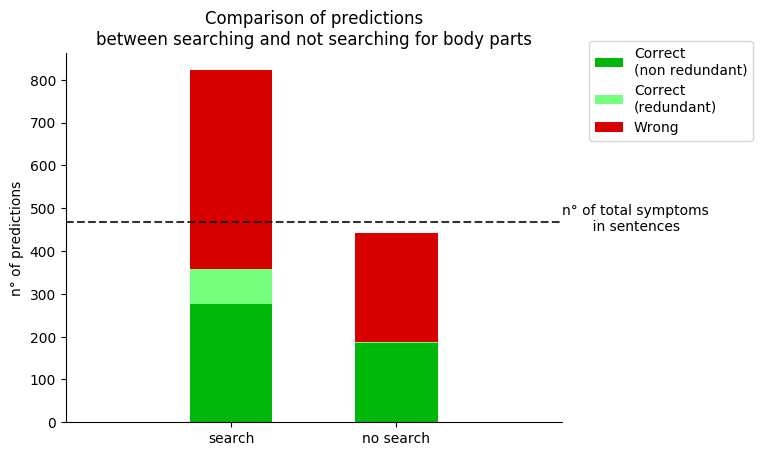
\includegraphics[width=9cm]{graphs/comparison_search_bp}
    \caption{Comparison of the composition of predictions when the Body Part Finder is enabled (\texttt{search}) and when it is not (\texttt{no search}).}
  \end{minipage}
  \hfill
  \begin{minipage}[b]{0.4\textwidth}
    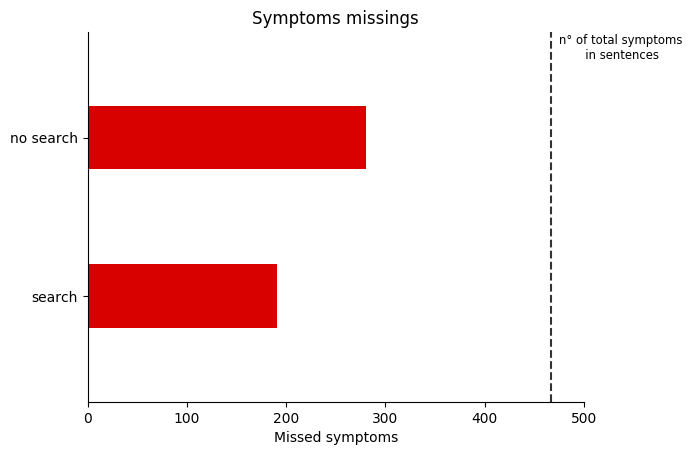
\includegraphics[width=8cm]{graphs/comparison_search_bp_missings}
    \caption{Comparison of the \texttt{missing symptoms} when the Body Part Finder is enabled (\texttt{search}) and when it is not (\texttt{no search}).}
  \end{minipage}
\end{figure}

\begin{center}
 \begin{tabular}{| c | c | c | c | c |} 
 \hline
  & \thead{\texttt{accuracy}} & \thead{\texttt{correct}\\\texttt{predictions}} & \thead{\texttt{medium}\\\texttt{attempts}} & \thead{\texttt{missed}\\\texttt{symptoms}} \\ [0.5ex] 
 \hline\hline
 \texttt{search} & 59.1 \% & 43.7 \% & 1.8 & 191 \\
 \hline
 \texttt{no search} & 39.8 \% & 42.2 \% & 0.9 & 281 \\
 \hline
\end{tabular}
\caption{Indexes comparison when the Body Part Finder is enabled (\texttt{search}) and when it is not (\texttt{no search}).}
\end{center}

%%%%%%%%%%%%%%%%%%%%%%%%%%% discuss data

The introduction of the Body Part Finder led to both pros and cons. The advantage is that there was a large improvement in accuracy (+ 19.3 \%). However, the downside of this percentage lift is that the \texttt{medium attempts} for each symptom in the sentences passed from 0.9 (where there was not enough tokens for predictions in order to cover the \texttt{\#real cuis}) to 1.8 (an excessive number of tokens for predictions).

The percentage of $\texttt{correct}^{\texttt{NR}}$ with respect to the total number of prediction decreased from 41.9 \% (\texttt{no search} for body parts) to 33.5 \% (\texttt{search} for body parts). This was caused by the lift of the number of wrong predictions, that were probably random classifications based on non-sense or wrong tokens for predictions. % For this reason the necessary future work is to limit non-sense tokens.

%%%%%%%%%%%%%%%%%%%%%%%%%%%

\newpage
\subsubsection{Ablation test for the ``pruning'' option}

\begin{figure}[h]%[!tbp]
  \centering
  \begin{minipage}[b]{0.4\textwidth}
    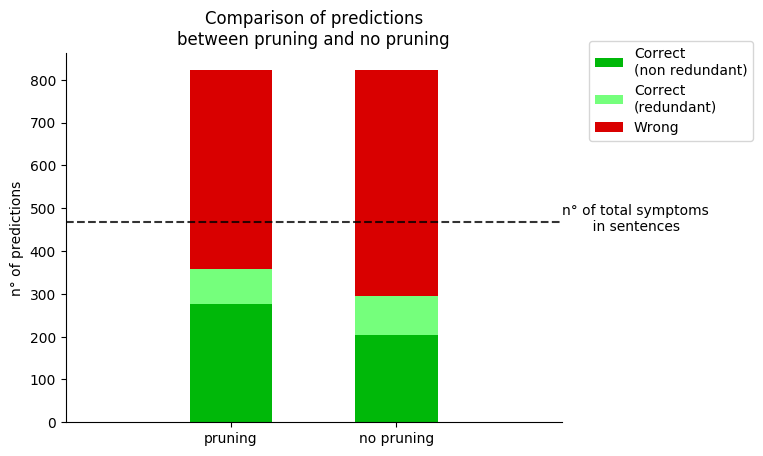
\includegraphics[width=9cm]{graphs/comparison_pruning}
    \caption{Comparison of the composition of predictions when the ``pruning'' option is enabled (\texttt{pruning}) and when it is not (\texttt{no pruning}).}
  \end{minipage}
  \hfill
  \begin{minipage}[b]{0.4\textwidth}
    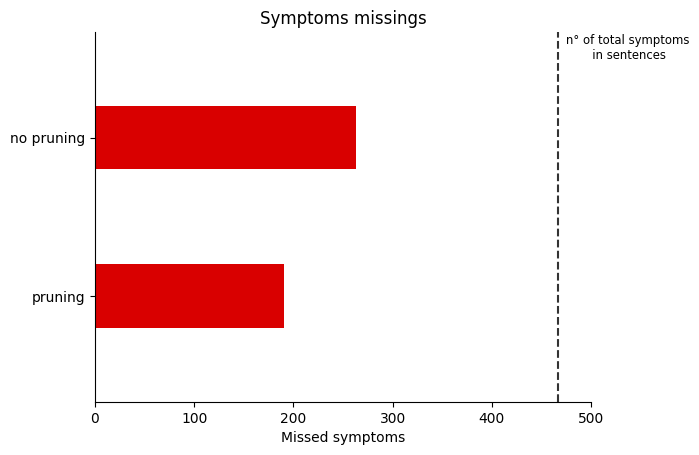
\includegraphics[width=8cm]{graphs/comparison_pruning_missings}
    \caption{Comparison of the \texttt{missing symptoms} when the ``pruning'' option is enabled (\texttt{pruning}) and when it is not (\texttt{no pruning}).}
  \end{minipage}
\end{figure}

\begin{center}
 \begin{tabular}{| c | c | c | c | c |} 
 \hline
  & \thead{\texttt{accuracy}} & \thead{\texttt{correct}\\\texttt{predictions}} & \thead{\texttt{medium}\\\texttt{attempts}} & \thead{\texttt{missed}\\\texttt{symptoms}} \\ [0.5ex] 
 \hline\hline
 \texttt{pruning} & 59.1 \% & 43.7 \% & 1.8 & 191 \\
 \hline
 \texttt{no pruning} & 43.7 \% & 36.0 \% & 1.8 & 263 \\
 \hline
\end{tabular}
\caption{Indexes comparison when the ``pruning'' option is enabled (\texttt{pruning}) and when it is not (\texttt{no pruning}).}
\end{center}

%%%%%%%%%%%%%%%%%%%%%%%%%%% discuss data

It is evident that this component contributes positively to the results. This because with the same number of predictions (the \texttt{medium attempts} score rests the same) its introduction causes an improvement in both \texttt{accuracy} (+ 15.4 \%) and \texttt{correct predictions} (+ 7.7 \%).

%%%%%%%%%%%%%%%%%%%%%%%%%%%

\newpage
\subsubsection{Ablation test for the filter of ``useless words''}
\begin{figure}[h]%[!tbp]
  \centering
  \begin{minipage}[b]{0.4\textwidth}
    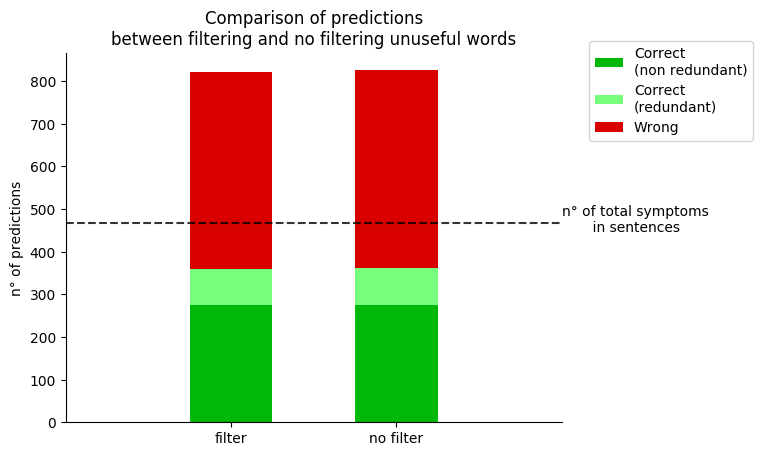
\includegraphics[width=9cm]{graphs/comparison_filtering}
    \caption{Comparison of the composition of predictions when the filtering ``useless words'' option is enabled (\texttt{filter}) and when it is not (\texttt{no filter}).}
  \end{minipage}
  \hfill
  \begin{minipage}[b]{0.4\textwidth}
    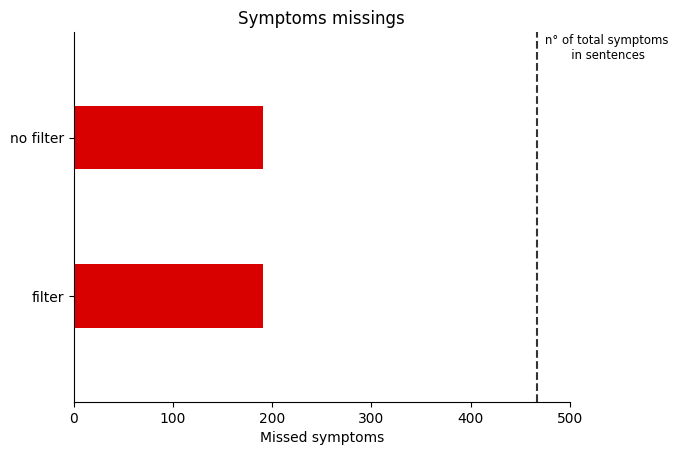
\includegraphics[width=8cm]{graphs/comparison_filtering_missings}
    \caption{Comparison of the \texttt{missing symptoms} when the filtering ``useless words'' option is enabled (\texttt{filter}) and when it is not (\texttt{no filter}).}
  \end{minipage}
\end{figure}

\begin{center}
 \begin{tabular}{| c | c | c | c | c |} 
 \hline
  & \thead{\texttt{accuracy}} & \thead{\texttt{correct}\\\texttt{predictions}} & \thead{\texttt{medium}\\\texttt{attempts}} & \thead{\texttt{missed}\\\texttt{symptoms}} \\ [0.5ex] 
 \hline\hline
 \texttt{filter} & 59.1 \% & 43.7 \% & 1.8 & 191 \\
 \hline
 \texttt{no filter} & 59.1 \% & 43.9 \% & 1.8 & 191 \\
 \hline
\end{tabular}
\caption{Indexes comparison when the filtering ``useless words'' option is enabled (\texttt{filter}) and when it is not (\texttt{no filter}).}
\end{center}

%%%%%%%%%%%%%%%%%%%%%%%%%%% discuss data

This option shows to be completely ineffective. This can be due to the fact that the Symptom Classifier considers all the possible subsentences of a token for prediction and maps the most similar to a symptom. This behavior already filters the so-called ``useless words'' because, generally, they are not used in the concept names of symptoms.

%%%%%%%%%%%%%%%%%%%%%%%%%%

\newpage
\subsubsection{Comparing different levels of \textit{minimum similarity}}
\begin{figure}[h]%[!tbp]
  \centering
  \begin{minipage}[b]{0.4\textwidth}
    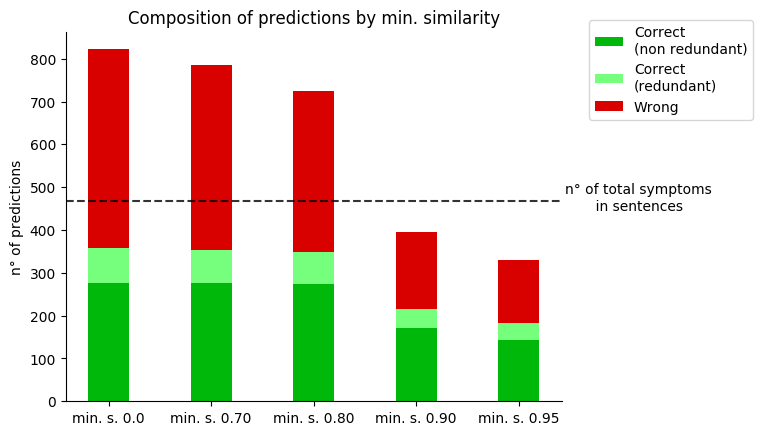
\includegraphics[width=9cm]{graphs/comparison_min_similarity}
    \caption{Comparison of the composition of predictions when different minimum similarity thresholds are used.}
  \end{minipage}
  \hfill
  \begin{minipage}[b]{0.4\textwidth}
    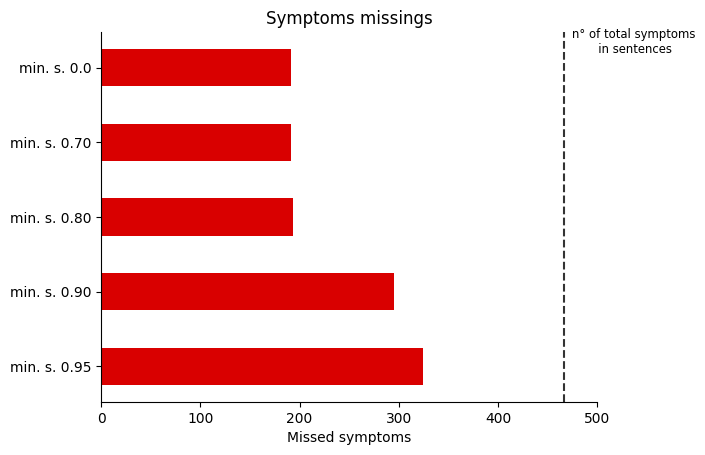
\includegraphics[width=8cm]{graphs/comparison_min_similarity_missings}
    \caption{Comparison of the \texttt{missing symptoms} when different minimum similarity thresholds are used.}
  \end{minipage}
\end{figure}

\begin{center}
 \begin{tabular}{| c | c | c | c | c |} 
 \hline
  \thead{\texttt{minimum}\\\texttt{similarity}} & \thead{\texttt{accuracy}} & \thead{\texttt{correct}\\\texttt{predictions}} & \thead{\texttt{medium}\\\texttt{attempts}} & \thead{\texttt{missed}\\\texttt{symptoms}} \\ [0.5ex] 
 \hline\hline
 \texttt{0.00} & 59.1 \% & 43.7 \% & 1.8 & 191 \\ 
 \hline
 \texttt{0.70} & 59.1 \% & 45.1 \% & 1.7 & 191 \\
 \hline
 \texttt{0.80} & 58.7 \% & 48.0 \% & 1.5 & 193 \\
 \hline
 \texttt{0.90} & 36.8 \% & 54.7 \% & 0.8 & 295 \\
 \hline
 \texttt{0.95} & 30.6 \% & 55.3 \% & 0.7 & 324 \\
 \hline
\end{tabular}
\caption{Indexes comparison when different minimum similarity thresholds are used.}
\label{tab:minsim}
\end{center}

%%%%%%%%%%%%%%%%%%%%%%%%%%% discuss data

The objective of this test is to examine if is possible to lower the \texttt{medium attempts} score without penalizing heavily the \texttt{accuracy}. As shown in the table \ref{tab:minsim}, it is possible to do it gradually raising the minimum similarity threshold. With this data, the best performance is gained with a $0.8$ level (the accuracy decreases by 0.4 \% meanwhile the medium attempts pass from $1.8$ to $1.5$ and the percentage of correct predictions lifts to 48.0 \%).

The found optimum minimum similarity level is not suitable for each dataset: this meta-parameter could be over-fitted to the examples. However, this test can be interpreted as a proof of concept for testing the effectiveness of this approach.

%%%%%%%%%%%%%%%%%%%%%%%%%%%
